\documentclass[11pt]{article}
\usepackage[paperwidth=8.5in, paperheight=11in]{geometry}

\usepackage{../tjimo}

\newcommand{\sevenpoints}{Time limit: 45 minutes.}
\newcommand{\righthead}{\fdbox{Round}{Team}}

\begin{document}

\section{Formatting}
Each problem is ranked 1-5 in terms of difficulty.

\section{Algebra}
\begin{problem}
(1.5) (2016azhang) Kangaskhan-Mega knows a move called Double Hit, which hits twice and deals $x$ damage per hit. However, Kangaskhan-Mega also has a special ability that allows it to use each move twice, with the second instance of the move dealing half damage. If Kangaskhan-Mega deals 105 damage in total using Double Hit and its special ability, find $x$.
\end{problem}

\begin{answer}
\boxed{35}.
\end{answer}

\begin{solution}
If Kangaskhan-Mega uses Double Hit without its special ability, it will deal $2x$ damage. With its special ability, it will deal $x$ additional damage. Thus, $2x + x = 105$, and we get $x = 35$.
\end{solution}

\begin{problem}
(2) (2016azhang) Cubone is chopping up a cube with side length 3 in. into 27 little cubes with side length 1 in. Find the minimum number of straight cuts this takes, if Cubone can rearrange pieces that have been chopped off in any manner.
\end{problem}

\begin{answer}
\boxed{6}.
\end{answer}

\begin{solution}
Cubone can chop the cube with side length 3 in. into 27 unit cubes with 6 straight cuts; imagine cutting up a Rubik's Cube. Thus we know our answer must be less than or equal to 6. However, note that the unit cube in the center of the 3 in. cube can only be obtained by at least 6 cuts, no matter how we rearrange the leftover pieces. Thus, the minimum number of cuts is 6 cuts.
\end{solution}


\begin{problem}
(3) (2016azhang) Ships Jendy and Sam6 are racing down a 500 km waterway. Jendy is going full speed ahead at 30 km/hr, but the captain of Sam6, Mr. Skim, is currently sleeping and has set the ship Sam6 on autopilot at 20 km/hr. When Mr. Skim wakes up, he instantly increases Sam6's speed to 45 km/hr in an effort to catch up. What is the maximum time in hours Mr. Skim can spend sleeping to be able to catch up to Jendy by the end of the race?
\end{problem}

\begin{answer}
\boxed{\frac{107}{13}}.
\end{answer}

\begin{solution}
We have that Jendy finishes in $\frac{500 \text{ km}}{30 \text{ km/hr}} = \frac{50}{3}$ hours, so Sam6 must also finish in $\frac{50}{3}$ hours in order to catch up to Jendy. Let $x$ denote the maximum time in hours that Mr. Skim can spend sleeping. Then, $\frac{50}{3} - x$ denotes the time in hours that Mr. Skim is awake and sailing Sam6 at 45 km/hr. Thus, we have that $20x + 45(\frac{50}{3}-x) = 500$. Solving gives us $x = \fbox{$\frac{107}{13}$}$.
\end{solution}

\begin{problem}
(5) (2016azhang) Compute $\sqrt{7+4\sqrt{3}} - \sqrt{7-4\sqrt{3}}$.
\end{problem}

\begin{answer}
\boxed{2\sqrt{3}}.
\end{answer}

\begin{solution}
Let $x = \sqrt{7+4\sqrt{3}} - \sqrt{7-4\sqrt{3}}$. Then $x^2 = (7+4\sqrt{3}) - 2\sqrt{(7+4\sqrt{3}(7-4\sqrt{3})} + (7-4\sqrt{3}) = 14 - 2\sqrt{1} = 12$. Since $x$ is positive by inspection, we take the positive square root to obtain $x = 2\sqrt{3}$.
\end{solution}

%-----------------------------------%
\section{Geometry}

\begin{problem}
(1.5) (2016skim) What is the area of the figure below, if it is made up of two overlapping squares of side length 10?
\begin{center}
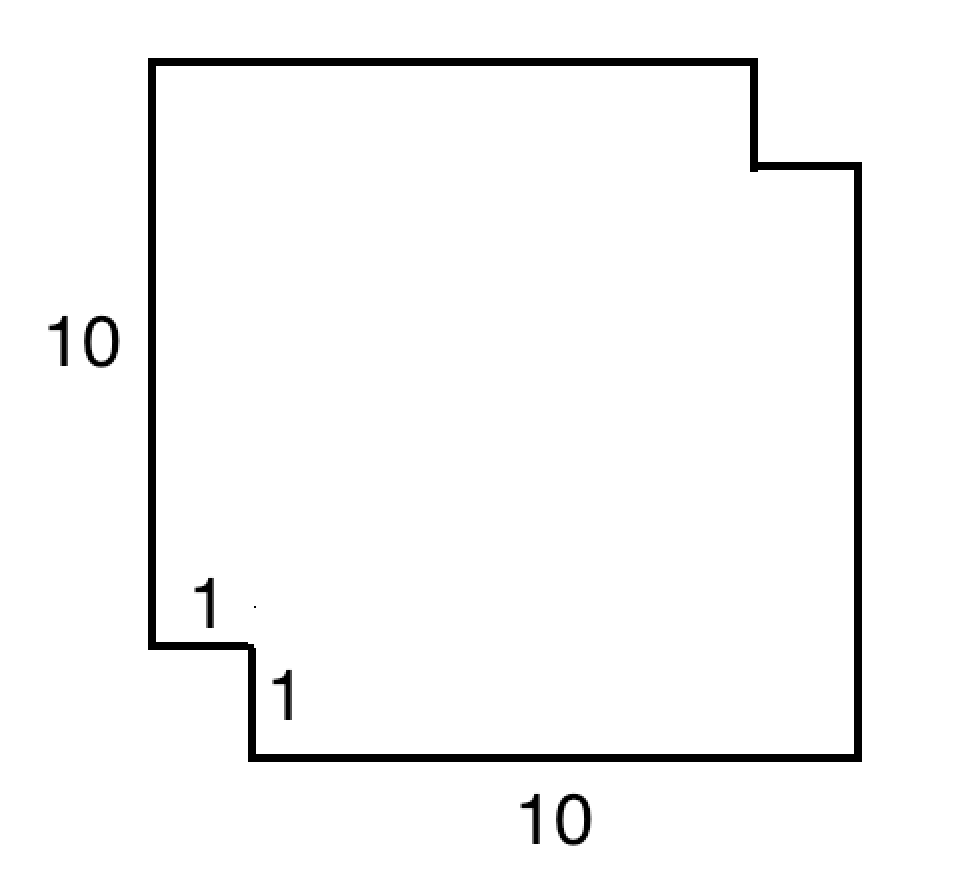
\includegraphics[width=9cm]{squares.png}
\end{center}
\end{problem}

\begin{answer}
\boxed{119}.
\end{answer}

\begin{solution}
We can view this as a $11\times11$ square with 2 unit squares cut off at the corners. The total area is $(11)(11)-2(1) = 119$.
\end{solution}


\begin{problem}
(3) (2016skim) If the area of the shaded area, made up of quarter-circles, is $16\pi$, what is the area of the nonshaded area?
\begin{center}
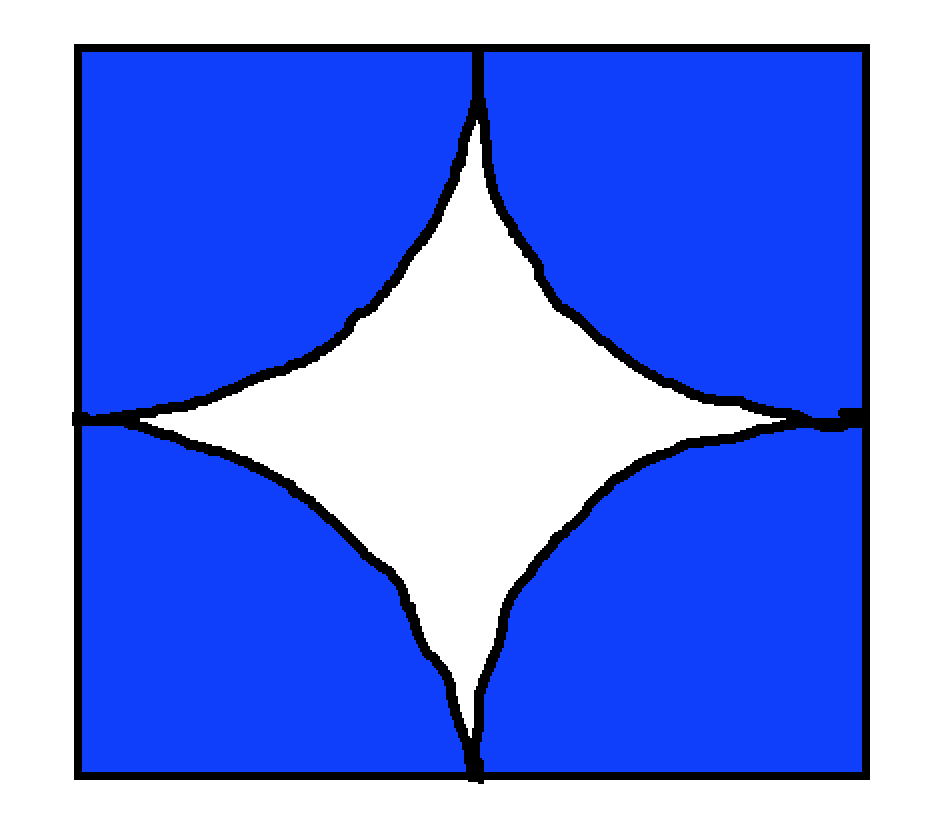
\includegraphics[width=9cm]{asteroid.png}
\end{center}
\end{problem}

\begin{answer}
\boxed{64 - 16\pi}.
\end{answer}

\begin{solution}
The shaded area is made up of 4 quarter-circles, which is equal to 1 circle of the same radius in area. Let the radius of this circle be $r$. Then $r^{2}\pi = 16\pi$, so $r = 4$. The nonshaded area is thus the area of a square with side length $2r = 8$ minus the shaded area, or $64 - 16\pi$.
\end{solution}


\begin{problem}
(2.5) (2016skim) If a triangle has an altitude of 12 from a side of 5, what is the altitude from a side of 10?
\end{problem}

\begin{answer}
\boxed{6}
\end{answer}

\begin{solution}
The area of a triangle is $\frac{1}{2} \cdot b \cdot h$. Looking at the base of 5, the area is
$\frac{1}{2} \cdot 5 \cdot 12 = 30$. Looking at the other pair, $\frac{1}{2} \cdot 10 \cdot h = 30$, so $h = 6$.
\end{solution}

%------------------------------%
\section{Combo}
\begin{problem}
(2016azhang) Pikachu is facing off against Blissey, who has a high special defense. Luckily, Pikachu knows the move Charge Beam, which has a 70 percent chance of boosting Pikachu's special attack by 1 stage. 

\begin{enumerate}
\item (1) If Pikachu uses Charge Beam 3 times, what is the probability that Pikachu's special attack will not be boosted at all?
\item (2.5) What is the probability that Pikachu gets 2 special attack boosts in 3 moves? 
\item (2.5) Find the expected number of special attack boosts Pikachu gets in 5 moves.
\item (4) What is the probability that Pikachu gets at least 2 special attack boosts in 4 moves?
\end{enumerate}
\end{problem}

\begin{problem}
\item (2.5) (2016skim) How many ways can you arrange six (distinct) people in a row, given that (person A) and (person B) have to be next to each other?
\end{problem}

\begin{answer}
\boxed{240}
\end{answer}

\begin{solution}
We can think of A and B as one person, since they need to be next to each other. This gives us $5! = 120$ ways of arranging them. We also need to multiply by 2 at the end to account for the arrangement of A and B: either AB or BA. This gives us $120\cdot2 = 240$.
\end{solution}


\begin{problem}
%(4) Kevlin and Kelvin are playing ERS, a card game played with a deck of 52 cards. They randomly split the deck, but if one person gets at least 5 more cards than the other person, the difference is noticeable. (What about 3 players?)

(4) (2016azhang) Kevlin and Kelvin are playing Monopoly with a slight twist. Instead of receiving \$1500 each at the beginning, they will receive a random real amount of money from \$0 to \$2000, determined by a computer. However, if the difference in money between them is over \$1800, they will run the computer randomizer again. What is the probability that they won't have to run the computer randomizer again? (Note: "random real amount of money" implies that \$1989.42425 can be earned; money is not limited to just cents.)
\end{problem}

\begin{answer}
\boxed{\frac{99}{100}}.
\end{answer}

\begin{solution}
\end{solution}

\section{NT}
\begin{problem}
(2) (2016azhang) Candide has 120 pieces of candy. In how many ways can Candide split all of his candies into equally sized pile(s)? (Two examples are 1 pile of 120 pieces, and 20 piles of 6 pieces.)
\end{problem}

\begin{answer}
\boxed{16}.
\end{answer}

\begin{solution}
Note that the number of piles (or the number of pieces in a pile) can only be a factor of 120. Since each number of piles leads to a unique pile distribution, our answer is just the number of factors of $120 = 2^{3}\cdot3\cdot5$, which is $(3+1)(1+1)(1+1) = 16$.
\end{solution}

\begin{problem}
(4) (2016azhang) Find the number of factors of 60300 that are divisible by 30.
\end{problem}

\begin{answer}
\boxed{16}.
\end{answer}

\begin{solution}
60300 has a prime factorization of $2^2\cdot3^2\cdot5^2\cdot67$. A factor of 60300 can only be the product of one number in every set of the following: $\{2^0, 2^1, 2^2\}, \{3^0, 3^1, 3^2\}, \{5^0, 5^1, 5^2\}$, and $\{67^0, 67^1\}$. For a factor to be divisible by $30 = 2\cdot3\cdot5$, we must choose $2^1$ or $2^2$ from the first set, $3^1$ or $3^2$ from the second set, and $5^1$ or $5^2$ from the third set; we can choose any number from the last set. Thus, our answer is $2\cdot2\cdot2\cdot2 = 16$.
\end{solution}

\section{Logic}
\begin{problem}
(4) (2018hkang) There are 4 boys who wish to ask Wendy to homecoming, Jeffrey, Jeff, Geoffrey, and Jeh-frey. However, among these 4 boys, there is only one truth-teller; the other three are liars. Only the truth-teller will actually ask Wendy to homecoming. 

Jeffrey says: "Jeh-frey is telling the truth."

Jeff says: "Jeffrey is a liar."

Geoffrey says: "Jeff is a liar."

Jeh-frey says: "I will ask Wendy to homecoming."

Which boy will ask Wendy to homecoming?
\end{problem}

\begin{answer}
\boxed{\text{Jeff}}.
\end{answer}

\begin{solution}
Assume that Jeffrey is the truth-teller. Then Jeff, Geoffrey, and Jeh-frey must be liars. Truth-teller Jeffrey says that Jeh-frey is telling the truth; but this is false based on our assumption above. Thus, Jeffrey must be a liar.

Next, assume that Jeff is the truth-teller. Then Jeffrey, Geoffrey, and Jeh-frey must be liars. Truth-teller Jeff says that Jeffrey is a liar, which is indeed true. Liar Jeffrey says that Jeh-frey is telling the truth, which is indeed false. Liar Geoffrey says that Jeff is a liar, which is indeed false. Finally, Liar Jeh-frey says that he will ask Wendy to homecoming, which is indeed false. Thus, we conclude that Jeff must be the truth-teller.
\end{solution}

\end{document}

